\begin{comment}
      \begin{figure*}
      \centering
      \begin{tabular}{@{}c@{\hspace{1mm}}c@{}}
          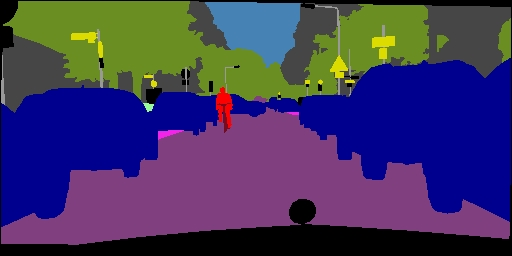
\includegraphics[width=0.493\textwidth]{figures/Label_000167.jpg} &
          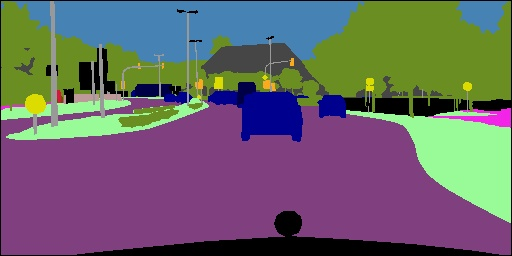
\includegraphics[width=0.493\textwidth]{figures/Label_000275.jpg}\vspace{0mm}\\
          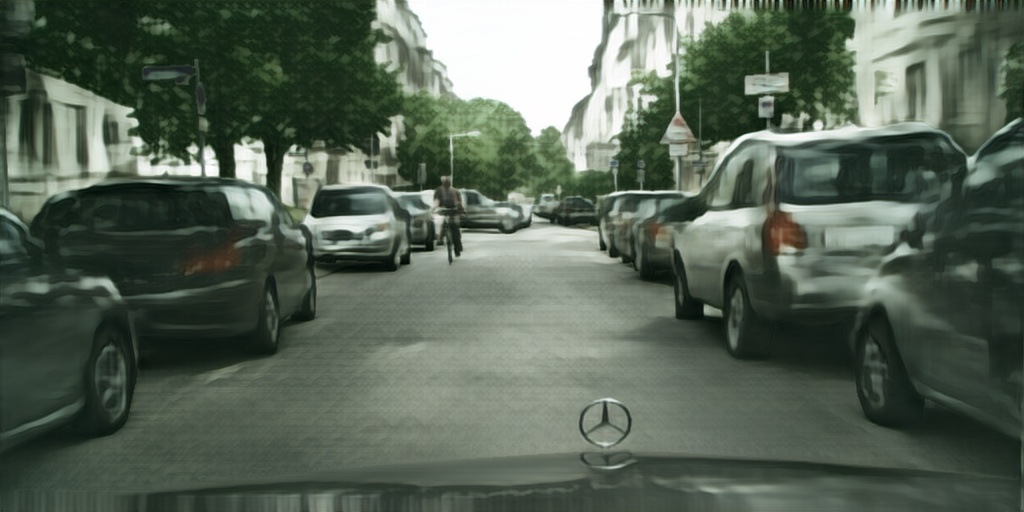
\includegraphics[width=0.493\textwidth]{figures/Ours_000167.jpg} &
          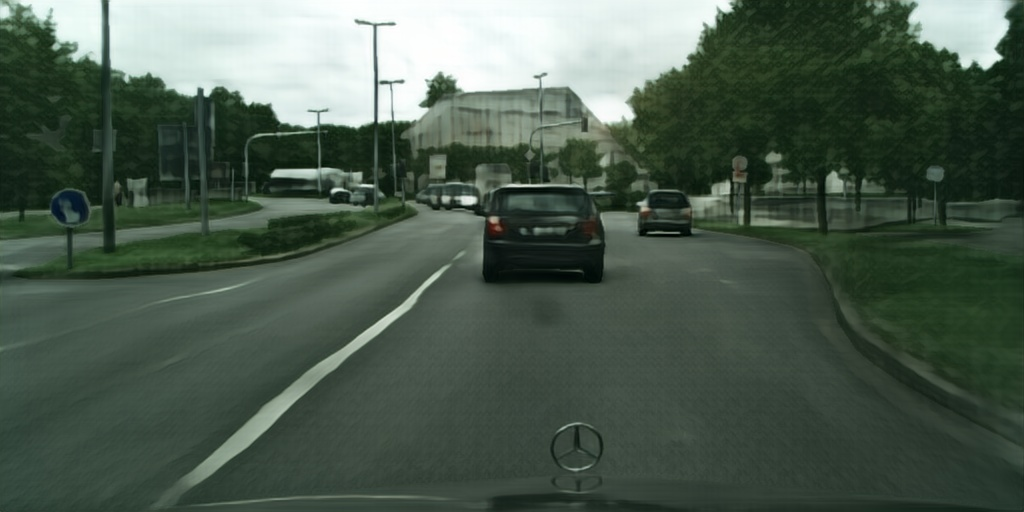
\includegraphics[width=0.493\textwidth]{figures/Ours_000275.jpg}\vspace{0mm}\\
          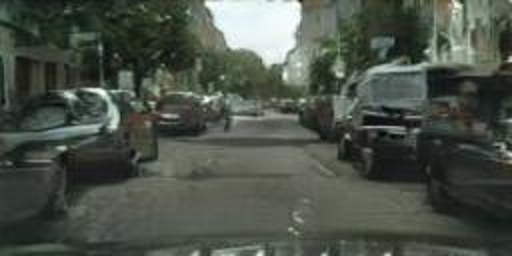
\includegraphics[width=0.493\textwidth]{figures/Bekeley_000167.jpg} &
          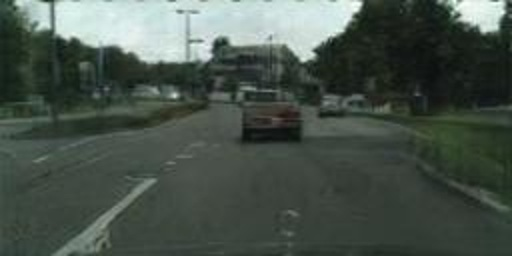
\includegraphics[width=0.493\textwidth]{figures/Bekeley_000275.jpg}
      \end{tabular}
      \vspace{2mm}
      \caption{Comparison.}
      \label{fig:comparison}
      \vspace{2mm}
      \end{figure*}

      \begin{figure*}
      \centering
      \begin{tabular}{@{}c@{\hspace{1mm}}c@{\hspace{1mm}}c@{}}
          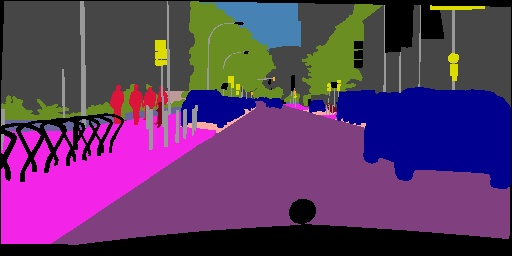
\includegraphics[width=0.330\textwidth]{figures/Label_000121.jpg} &
          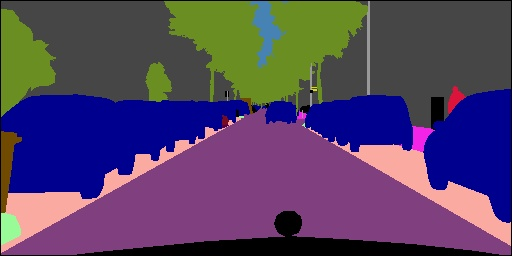
\includegraphics[width=0.330\textwidth]{figures/Label_000343.jpg} &
          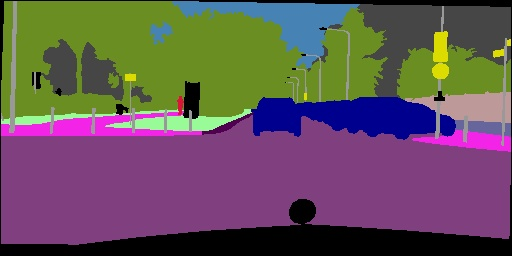
\includegraphics[width=0.330\textwidth]{figures/Label_000245.jpg}\vspace{0mm}\\
          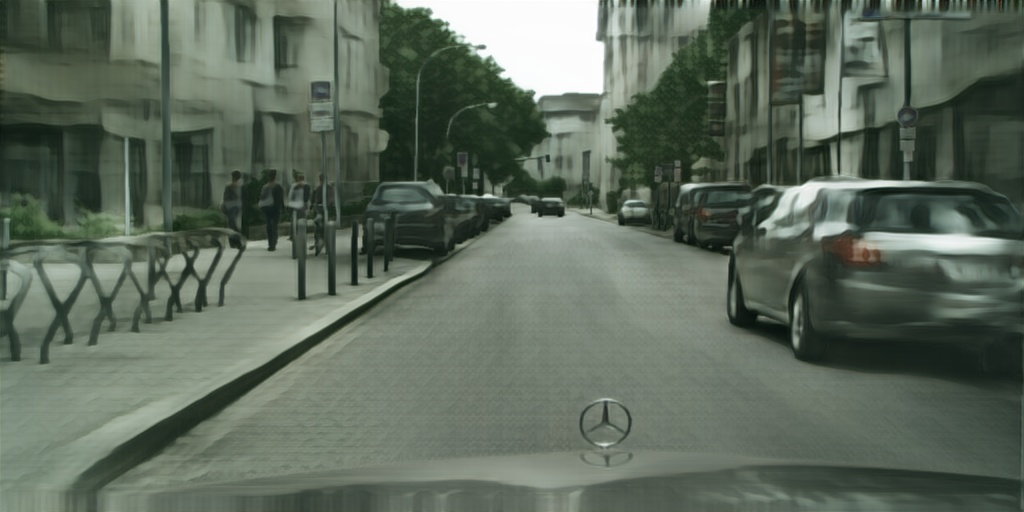
\includegraphics[width=0.330\textwidth]{figures/Ours_000121.jpg} &
          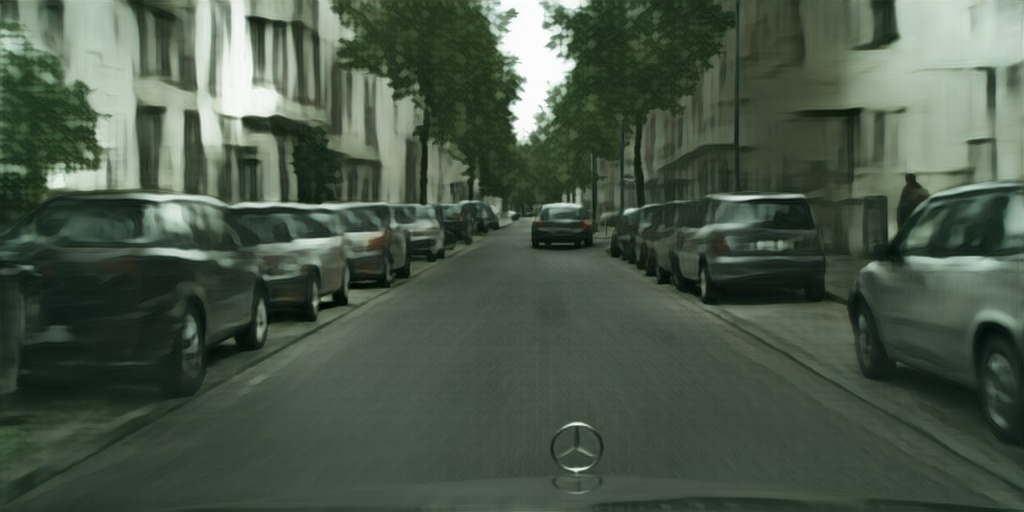
\includegraphics[width=0.330\textwidth]{figures/Ours_000343.jpg} &
          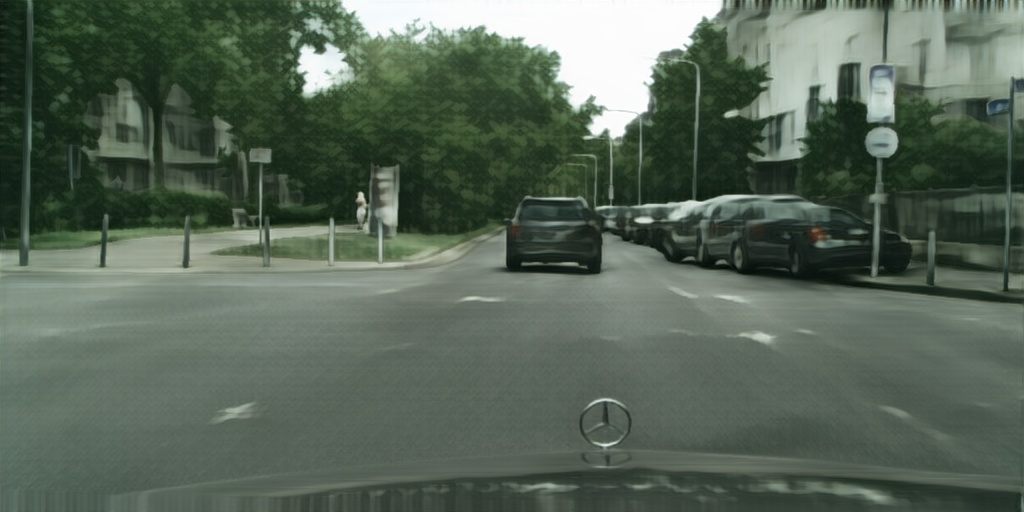
\includegraphics[width=0.330\textwidth]{figures/Ours_000245.jpg}\vspace{0mm}\\
          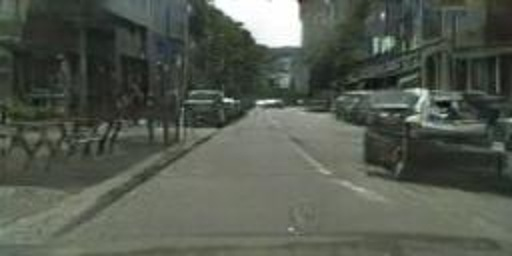
\includegraphics[width=0.330\textwidth]{figures/Bekeley_000121.jpg} &
          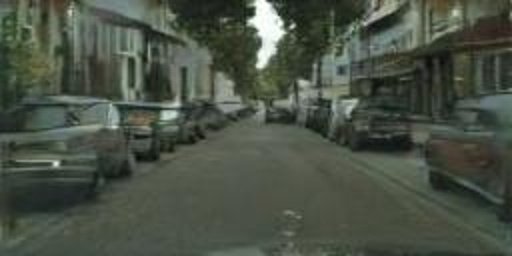
\includegraphics[width=0.330\textwidth]{figures/Bekeley_000343.jpg} &
          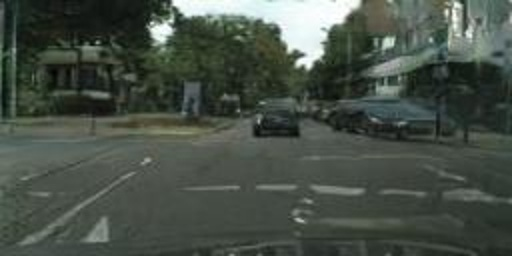
\includegraphics[width=0.330\textwidth]{figures/Bekeley_000245.jpg}
      \end{tabular}
      \vspace{2mm}
      \caption{Comparison.}
      \label{fig:comparison}
      \vspace{2mm}
      \end{figure*}
\end{comment}

\begin{figure*}[t]
\centering
\begin{tabular}{@{}c@{\hspace{2mm}}c@{\hspace{2mm}}c@{}}
\rotatebox{90}{\hspace{11mm}Input layout}&
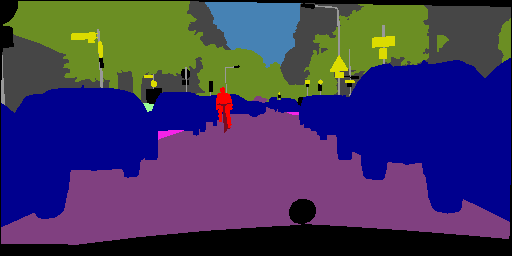
\includegraphics[width=0.46\linewidth]{figures/Label_000167.png} &
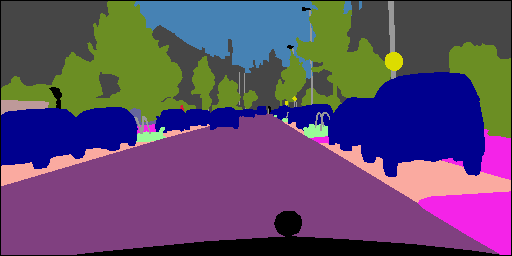
\includegraphics[width=0.46\linewidth]{figures/Label_000437.png}\\
\rotatebox{90}{\hspace{12.5mm}Our result}&
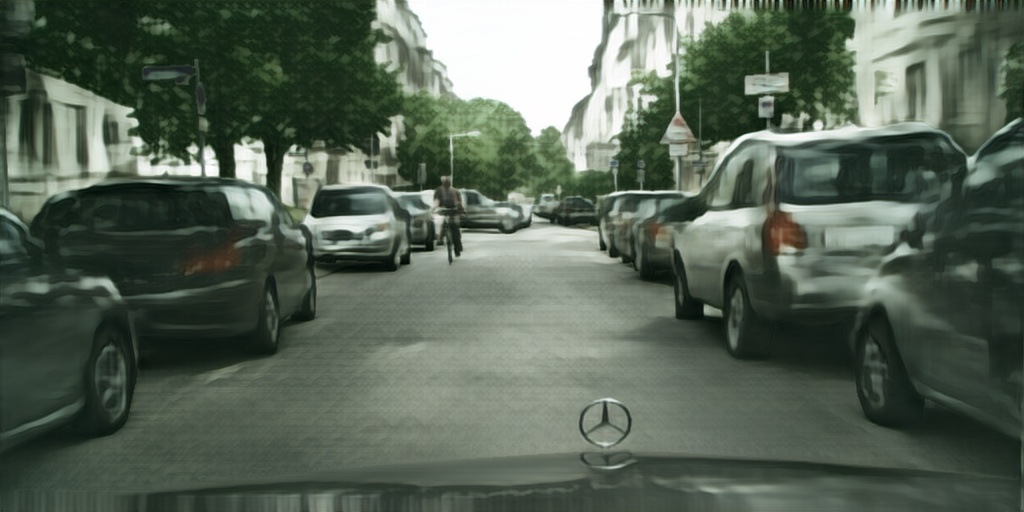
\includegraphics[width=0.46\linewidth]{figures/Ours_000167.jpg}&
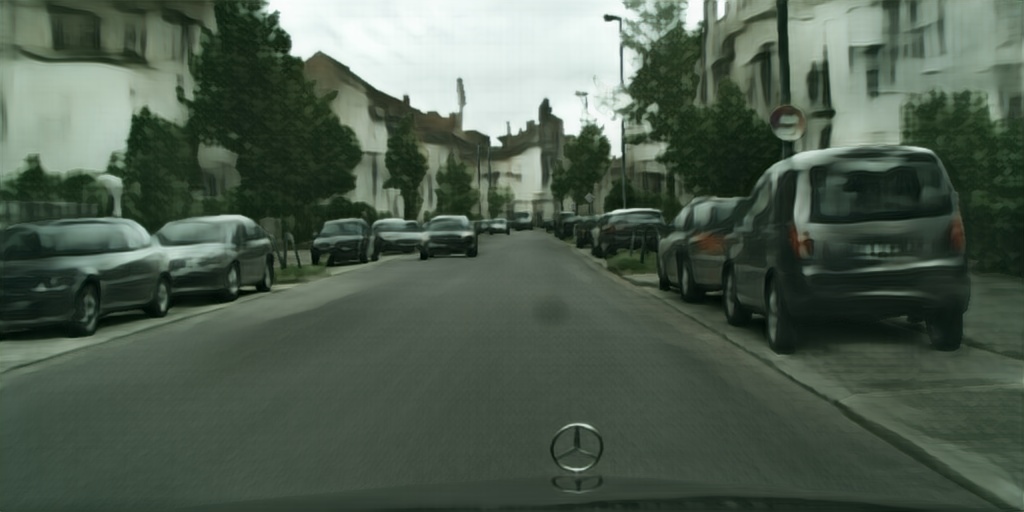
\includegraphics[width=0.46\linewidth]{figures/Ours_000437.jpg} \\
\rotatebox{90}{\hspace{12mm}Isola et al.}&
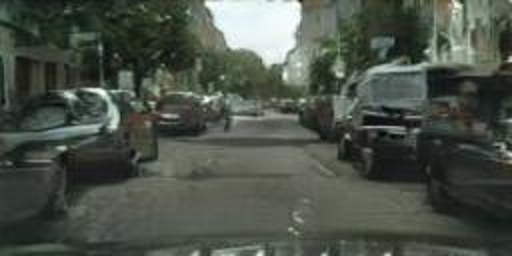
\includegraphics[width=0.46\linewidth]{figures/Bekeley_000167.jpg}&
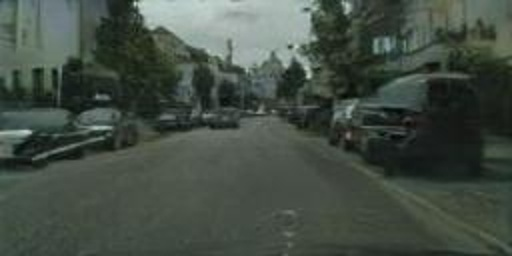
\includegraphics[width=0.46\linewidth]{figures/Bekeley_000437.jpg}
\end{tabular}
\vspace{0.5mm}
\caption{Comparison to the approach of Isola et al.~\cite{Isola2017}. Zoom in for details.}
\label{fig:comparison}
\vspace{-1mm}
\end{figure*}

The most prominent contemporary approach to image synthesis is based on generative adversarial networks (GANs)~\cite{Goodfellow2014}. In the original work of Goodfellow et al.~\cite{Goodfellow2014}, GANs were used to synthesize MNIST digits and $32\timess 32$ images that aimed to reproduce the appearance of different classes in the CIFAR-10 dataset. Denton et al.~\cite{Denton2015} proposed training multiple separate GANs, one for each level in a Laplacian pyramid. Each model is trained independently to synthesize details at its scale. Assembling separately-trained models in this fashion enabled the authors to synthesize smoother images and to push resolution up to $96\timess 96$.
%multiple GANs chained in this fashion can synthesize smoother images and were able to push resolution up to $96\timess 96$.
%conditioned on the output from a lower level and is responsible for synthesizing details at its scale. Denton et al.~\cite{} showed that multiple GANs chained in this fashion can synthesize smoother images and were able to push resolution up to $96\timess 96$. Their work
This work is an important precursor to ours in that multi-scale refinement is a central characteristic of our approach. Key differences are that we train a single model end-to-end to directly synthesize the output image, and that no adversarial training is used.
%This allows us to go much further in resolution and realism.
%use a single model that is trained end-to-end through all scales.

Radford et al.~\cite{Radford2016} remark that ``Historical attempts to scale up GANs using CNNs to model images have been unsuccessful'' and describe a number of modifications that enable scaling up adversarial training to $64\timess 64$ images. Salimans et al.~\cite{Salimans2016} also tackle the instability of GAN training and describe a number of heuristics that encourage convergence. The authors synthesize $128\timess 128$ images that possess plausible low-level statistics.
%but no realistic structure.
%demonstrate image synthesis at $128\timess 128$ resolution,
%These adaptations allow the authors to synthesize $128\timess 128$ images, although
Nevertheless, as observed in recent work and widely known in the folklore, GANs ``remain remarkably difficult to train'' and ``approaches to attacking this problem still rely on heuristics that are extremely sensitive to modifications''~\cite{ArjovskyBottou2017}. (See also~\cite{Metz2017}.) Our work demonstrates that these difficulties can be avoided in the setting we consider.
%GANs are not necessary for synthesizing realistic high-resolution images from semantic layouts.

Dosovitskiy et al.~\cite{Dosovitskiy2016} train a ConvNet to generate images of 3D models, given a model ID and viewpoint. The network thus acts directly as a rendering engine for the 3D model. This is also an important precursor to our work as it uses direct feedforward synthesis through a network trained with a regression loss. Our model, loss, and problem setting are different, enabling synthesis of sharper higher-resolution images of scenes without 3D models.

Dosovitskiy and Brox~\cite{DosovitskiyBrox2016} introduced a family of composite loss functions for image synthesis, which combine regression over the activations of a fixed ``perceiver'' network with a GAN loss. Networks trained using these composite loss functions were applied to synthesize preimages that induce desired excitation patterns in image classification models~\cite{DosovitskiyBrox2016} and images that excite specific elements in such models~\cite{Nguyen2016}. In recent work, networks trained using these losses were applied to generate diverse sets of $227\timess 227$ images, to synthesize images for given captions, and to inpaint missing regions~\cite{Nguyen2017}. These works all rely on the aforementioned composite losses, which require balancing the adversarial loss with a regression loss. Our work differs in that GANs are not used, which simplifies the training procedure, architecture, and loss.
%Without the need to balance discordant objective terms, train multiple networks, and contend with unstable training dynamics, we are able to train much larger networks end-to-end and to synthesize HD images of scenes with given layouts.

%During the course of our research,
Isola et al.~\cite{Isola2017} consider a family of problems that include the image synthesis problem we focus on. The paper of Isola et al.~appeared on arXiv during the course of our research.
% and contemporaneous, and is not considered prior work. Nevertheless,
It provides an opportunity to compare our approach to a credible alternative that was independently tested on the same data. Like a number of aforementioned formulations, Isola et al.~use a composite loss that combines a GAN and a regression term.
%This composition suffers from the issues we reviewed.
The authors use the Cityscapes dataset and synthesize $256\timess 256$ images for given semantic layouts.
%, although 2-megapixel data is available. We believe
In comparison, our simpler direct formulation yields much more realistic images and scales seamlessly to high resolutions.
%enables training much larger models that synthesize more than an order of magnitude larger images that are significantly more realistic.
A qualitative comparison is shown in Figure~\ref{fig:comparison}.
% and quantitative experiments will be reported in Section~\ref{sec:experiments}.

Reed et al.~\cite{Reed2016:ICML} synthesize $64\timess 64$ images of scenes that are described by given sentences. Mansimov et al.~\cite{Mansimov2015} describe a different model that generates $32\timess 32$ images that aim to fit sentences. Yan et al.~\cite{Yan2016:ECCV} generate $64\timess 64$ images of faces and birds with given attributes. Reed et al.~\cite{Reed2016:NIPS} synthesize $128\timess 128$ images of birds and people conditioned on text descriptions and on spatial constraints such as bounding boxes or keypoints. Wang and Gupta~\cite{WangGupta2016} synthesize $128\timess 128$ images of indoor scenes by factorizing the image generation process into synthesis of a normal map and subsequent synthesis of a corresponding color image. Most of these works use GANs, with the exception of Yan et al.~\cite{Yan2016:ECCV} who use variational autoencoders and Mansimov et al.~\cite{Mansimov2015} who use a recurrent attention-based model~\cite{Gregor2015}. Our problem statement is different in that our input is a pixelwise semantic layout, and our technical approach differs substantially in that a single feedforward convolutional network is trained end-to-end to synthesize a high-resolution image.
%Our formulation is substantially different, as is our input (a pixelwise semantic layout).

A line of work considers synthesis of future frames in video. Srivastava et al.~\cite{Srivastava2015} train a recurrent network for this purpose. Mathieu et al.~\cite{Mathieu2016} build on the work of Denton et al.~\cite{Denton2015} and use a composite loss that combines an adversarial term with regression penalties on colors and gradients. Oh et al.~\cite{Oh2015} predict future frames in Atari games conditioned on the player's action. Finn et al.~\cite{Finn2016} explicitly model pixel motion and also condition on action. Vondrick et al.~\cite{Vondrick2016} learn a model of scene dynamics and use it to synthesize video sequences from single images. Xue et al.~\cite{Xue2016} develop a probabilistic model that enables synthesizing multiple plausible video sequences. In these works, a color image is available as a starting point for synthesis. Video synthesis can be accomplished by advecting the content of this initial image.
% in a Lagrangian~\cite{Finn2016} or an Eulerian~\cite{Xue2016} scheme.
In our setting, photographic scene appearance must be synthesized without such initialization.
% from segmentation and semantic cues alone.

Researchers have also studied image inpainting~\cite{Pathak2016}, superresolution~\cite{Bruna2016,Johnson2016,Ledig2016}, novel view synthesis~\cite{Flynn2016,Tatarchenko2016,Zhou2016}, and interactive image manipulation~\cite{Zhu2016}. In these problems, photographic content is given as input, whereas we are concerned with synthesizing photographic images from semantic layouts alone.
